% !TEX encoding = UTF-8
% !TEX TS-program = pdflatex
% !TEX root = ../tesi.tex

%**************************************************************
\chapter{Descrizione dettagliata dei casi d'uso}
\label{cap:appendice a}
%**************************************************************
In questa sezione verranno descritte tutti i casi d'uso dettagliamente.
La descrizione generale dei casi d'uso è reperibile alla sezione 3.2.\\

% \epigraph{Citazione}{Autore della citazione}
\textbf{Utente generico}\\
\textbf{UC1 - Visualizza menù}
\begin{figure}[H]
    \centering
    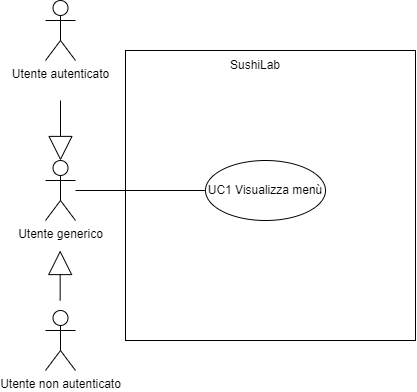
\includegraphics[scale=0.5]{usecase/tesi-uc1.drawio.png}
    \caption{Use Case - UC 1}
\end{figure}
\begin{itemize}
    \item \textbf{Descrizione:} L'utente visualizza il menù del ristorante.
    \item \textbf{Attore Primario:}L'utente generico.
    \item \textbf{Precondizione:} L'utente si trova dentro la web-app sushiLab.
    \item \textbf{Postcondizione:} Viene visualizzato il menù del ristorante.
    \item \textbf{Scenrio principale:}
    \begin{itemize}
        \item L'utente si trova dentro il sistema;
        \item L'utente clicca sul bottone menù;
        \item Viene mostra il menù del ristorante.
    \end{itemize}
\end{itemize}
\textbf{UC1.1 - Visualizza categorie}
\begin{figure}[H]
    \centering
    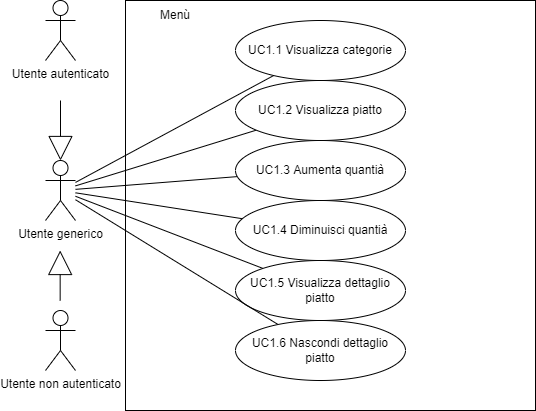
\includegraphics[scale=0.5]{usecase/tesi-uc11.drawio.png}
    \caption{Use Case - UC 1.1, UC 1.2, UC 1.3, UC 1.4, UC 1.5, UC 1.6}
\end{figure}
\begin{itemize}
    \item \textbf{Descrizione:} L'utente visualizza le categorie del menù.
    \item \textbf{Attore Primario:}L'utente generico.
    \item \textbf{Precondizione:} L'utente si trova dentro la sezione menù.
    \item \textbf{Postcondizione:} Viene visualizzato i nomi delle categorie.
    \item \textbf{Scenrio principale:}
    \begin{itemize}
        \item L'utente si trova sezione menù;
        \item Viene mostrato le categorie del menù.
    \end{itemize}
\end{itemize}
\textbf{UC1.2 - Visualizza piatto}
\begin{itemize}
    \item \textbf{Descrizione:} L'utente visualizza i piatti del menù mostrando il numero, nome, prezzo, ingredienti, allergeni, limatazioni e la quantità. La quantità di default è 0 che indica che non è ancora stato ordinato.
    \item \textbf{Attore Primario:}L'utente generico.
    \item \textbf{Precondizione:} L'utente si trova dentro la sezione menù.
    \item \textbf{Postcondizione:} Viene visualizzato i piatti del menù.
    \item \textbf{Scenrio principale:}  
    \begin{itemize}
        \item L'utente si trova sezione menù;
        \item Viene mostrato i piatti del menù.
    \end{itemize}
\end{itemize}
\textbf{UC1.3 - Aumenta quantità}
\begin{itemize}
    \item \textbf{Descrizione:} L'utente aumenta la quantità di un piatto.
    \item \textbf{Attore Primario:}L'utente generico.
    \item \textbf{Precondizione:} L'utente si trova dentro la sezione menù o lista degli ordini personali.
    \item \textbf{Postcondizione:} Viene aggiunto il piatto specifico con la quantità aggiornata negli ordini.
    \item \textbf{Scenrio principale:}
    \begin{itemize}
        \item L'utente si trova sezione menù;
        \item L'utente clicca sul bottone + di un piatto;
        \item Viene aggiunto il piatto negli ordini.
    \end{itemize}
    \item \textbf{Scenrio alternativo:}
    \begin{itemize}
        \item L'utente si trova sezione menù o lista degli ordini personali;
        \item L'utente clicca sul bottone + di un piatto che è già presente negli ordini;
        \item Viene aumentato la quantità del piatto negli ordini.
    \end{itemize}
\end{itemize}
\textbf{UC1.4 - Diminuisci quantità}
\begin{itemize}
    \item \textbf{Descrizione:} L'utente dimiuisce la quantità di un piatto.
    \item \textbf{Attore Primario:}L'utente generico.
    \item \textbf{Precondizione:} L'utente si trova dentro la sezione menù o lista degli ordini personali.
    \item \textbf{Postcondizione:} Viene dimiuito la quantità del piatto specifico negli ordini.
    \item \textbf{Scenrio principale:}
    \begin{itemize}
        \item L'utente si trova sezione menù o lista degli ordini personali;
        \item L'utente clicca sul bottone - di un piatto con quantità maggiore di 1;
        \item Viene diminuito la quantità del piatto negli ordini.
    \end{itemize}
    \item \textbf{Scenrio alternativo:}
    \begin{itemize}
        \item L'utente si trova sezione menù o lista degli ordini personali;
        \item L'utente clicca sul bottone - di un piatto con quantità uguale a 1;
        \item Viene rimosso il piatto dagli ordini.
    \end{itemize}
\end{itemize}
\textbf{UC1.5 - Visualizza dettaglio piatto}
\begin{itemize}
    \item \textbf{Descrizione:} L'utente visualizza i dettagli di un piatto nel menù, mostrando la recensione del piatto e il text-box per inserire una nota.
    \item \textbf{Attore Primario:}L'utente generico.
    \item \textbf{Precondizione:} L'utente si trova dentro la sezione menù.
    \item \textbf{Postcondizione:} Viene visualizzato i dettagli di un piatto specifico.
    \item \textbf{Scenrio principale:}  
    \begin{itemize}
        \item L'utente si trova sezione menù;
        \item L'utente clicca sul bottom mostra dettagli;
        \item Viene mostrato i dettagli di un piatto.
    \end{itemize}
\end{itemize}
\textbf{UC1.6 - Nascondi dettaglio piatto}
\begin{itemize}
    \item \textbf{Descrizione:} L'utente nasconde i dettagli di un piatto specifico.
    \item \textbf{Attore Primario:}L'utente generico.
    \item \textbf{Precondizione:} L'utente si trova dentro la sezione menù con un piatto in modalità dettaglio.
    \item \textbf{Postcondizione:} Viene nascosto i dettagli del piatto specifico.
    \item \textbf{Scenrio principale:}  
    \begin{itemize}
        \item L'utente si trova sezione menù;
        \item L'utente clicca sul bottom nascondi dettagli;
        \item Viene nascosto i dettagli del piatto.
    \end{itemize}
\end{itemize}
\textbf{UC2 - Gestione tavolo}
\begin{figure}[H]
    \centering
    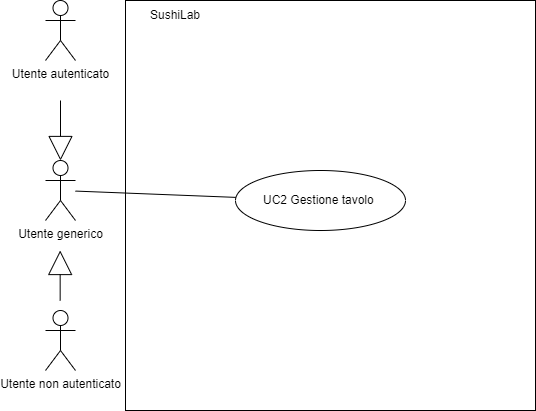
\includegraphics[scale=0.5]{usecase/tesi-uc2.drawio.png}
    \caption{Use Case - UC 2}
\end{figure}
\begin{itemize}
    \item \textbf{Descrizione:} L'utente visualizza la maschera di gestione tavolo.
    \item \textbf{Attore Primario:}L'utente generico.
    \item \textbf{Precondizione:} L'utente si trova dentro la web-app sushiLab.
    \item \textbf{Postcondizione:} Viene visualizzato la maschera di gestione tavolo.
    \item \textbf{Scenrio principale:}
    \begin{itemize}
        \item L'utente si trova dentro il sistema;
        \item L'utente clicca sul bottone gestione tavolo nella navbar;
        \item Viene mostrato la maschera di gestione tavolo.
    \end{itemize}
\end{itemize}
\textbf{UC2.1 - Generazione sessione tavolo}
\begin{figure}[H]
    \centering
    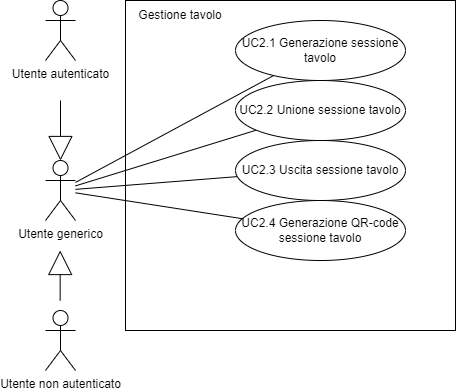
\includegraphics[scale=0.5]{usecase/tesi-uc21.drawio.png}
    \caption{Use Case - UC 2.1, UC 2.2, UC 2.3, UC 2.4}
\end{figure}
\begin{itemize}
    \item \textbf{Descrizione:} L'utente genera la sessione del tavolo.
    \item \textbf{Attore Primario:}L'utente generico.
    \item \textbf{Precondizione:} L'utente si trova dentro la sezione gestione tavolo.
    \item \textbf{Postcondizione:} L'utente entra nella sessione generata del tavolo.
    \item \textbf{Scenrio principale:}
    \begin{itemize}
        \item L'utente si trova dentro la sezione gestione tavolo;
        \item L'utente clicca sul bottone crea sessione;
        \item Viene creata la sessione;
        \item L'utente viene inserito nella sessione creata.
    \end{itemize}
\end{itemize}
\textbf{UC2.2 - Unione sessione tavolo}
\begin{itemize}
    \item \textbf{Descrizione:} L'utente si unisce alla sessione del tavolo.
    \item \textbf{Attore Primario:}L'utente generico.
    \item \textbf{Precondizione:} L'utente si trova dentro la sezione gestione tavolo.
    \item \textbf{Postcondizione:} L'utente entra nella sessione che è stata inserita.
    \item \textbf{Scenrio principale:}
    \begin{itemize}
        \item L'utente si trova dentro la sezione gestione tavolo;
        \item L'utente clicca sul bottone unisciti a una sessione;
        \item L'utente inserisce il numero della sessione;
        \item L'utente clicca sul bottone unisciti;
        \item L'utente viene inserito nella sessione.
    \end{itemize}
    % \item \textbf{Scenrio alternativo:}
    % \begin{itemize}
    %     \item L'utente si trova dentro la sezione gestione tavolo;
    %     \item L'utente clicca sul bottone unisciti a una sessione;
    %     \item L'utente inserisce il numero della sessione inesistente;
    %     \item L'utente clicca sul bottone unisciti;
    %     \item L'utente non viene inserito nella sessione.
    % \end{itemize}
\end{itemize}
\textbf{UC2.3 - Uscita sessione tavolo}
\begin{itemize}
    \item \textbf{Descrizione:} L'utente esce dalla sessione del tavolo.
    \item \textbf{Attore Primario:}L'utente generico.
    \item \textbf{Precondizione:} L'utente si trova dentro la sezione gestione tavolo ed è dentro ad una sessione.
    \item \textbf{Postcondizione:} L'utente esce dalla sessione generata del tavolo.
    \item \textbf{Scenrio principale:}
    \begin{itemize}
        \item L'utente si trova dentro la sezione gestione tavolo;
        \item L'utente clicca sul bottone esci dalla sessione;
        \item L'utente viene rimosso dalla sessione.
    \end{itemize}
\end{itemize}
\textbf{UC2.4 - Generazione QR-code sessione tavolo}
\begin{itemize}
    \item \textbf{Descrizione:} L'utente genera il QR-code dalla sessione del tavolo per mostrarlo agli altri, che li permetterà di unire alla sessione direttamente scansionando il QR-code.
    \item \textbf{Attore Primario:}L'utente generico.
    \item \textbf{Precondizione:} L'utente si trova dentro la sezione gestione tavolo ed è dentro ad una sessione.
    \item \textbf{Postcondizione:} L'utente genera il QR-code dalla sessione del tavolo.
    \item \textbf{Scenrio principale:}
    \begin{itemize}
        \item L'utente si trova dentro la sezione gestione tavolo;
        \item L'utente genera il QR-code della sessione;
        \item Vine mostrato il QR-code;
    \end{itemize}
\end{itemize}



\textbf{UC3 - Lista ordini}
\begin{figure}[H]
    \centering
    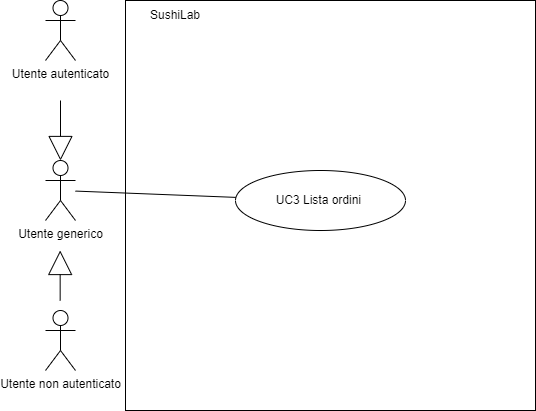
\includegraphics[scale=0.5]{usecase/tesi-uc3.drawio.png}
    \caption{Use Case - UC 3}
\end{figure}
\begin{itemize}
    \item \textbf{Descrizione:} L'utente visualizza la maschera di gestione ordini.
    \item \textbf{Attore Primario:}L'utente generico.
    \item \textbf{Precondizione:} L'utente si trova dentro ad una sessione di tavolo.
    \item \textbf{Postcondizione:} Viene visualizzato la maschera di gestione ordini.
    \item \textbf{Scenrio principale:}
    \begin{itemize}
        \item L'utente si trova dentro il sistema con una sessione di tavolo attiva;
        \item L'utente clicca sul bottone lista ordini nella navbar;
        \item Viene mostrato la maschera di gestione ordini.
    \end{itemize}
\end{itemize}
\textbf{UC3.1 - Visualizza lista ordini del tavolo}
\begin{figure}[H]
    \centering
    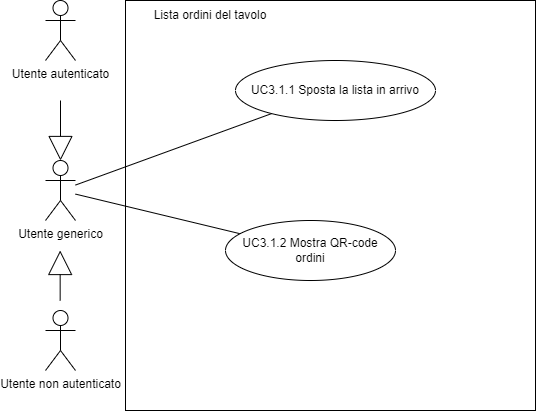
\includegraphics[scale=0.5]{usecase/tesi-uc311.drawio.png}
    \caption{Use Case - UC 3.1, UC 3.2, UC 3.3}
\end{figure}
\begin{itemize}
    \item \textbf{Descrizione:} L'utente visualizza la lista degli ordini della sessione di tavolo in cui si trova. 
    \item \textbf{Attore Primario:}L'utente generico.
    \item \textbf{Precondizione:} L'utente si trova dentro la sezione lista ordini.
    \item \textbf{Postcondizione:} Viene visualizzato la lista degli ordini del tavolo.
    \item \textbf{Scenrio principale:}
    \begin{itemize}
        \item L'utente si trova dentro la sezione gestione ordini;
        \item L'utente clicca sul bottone "tavolo";
        \item Viene mostrato la lista dei piatti ordinati del tavolo.
    \end{itemize}
\end{itemize}
\textbf{UC3.2 - Visualizza lista ordini personali}
\begin{itemize}
    \item \textbf{Descrizione:} L'utente visualizzato la lista degli ordini personali.
    \item \textbf{Attore Primario:}L'utente generico.
    \item \textbf{Precondizione:} L'utente si trova dentro la sezione lista ordini.
    \item \textbf{Postcondizione:} Viene visualizzato la lista degli ordini personali.
    \item \textbf{Scenrio principale:}
    \begin{itemize}
        \item L'utente si trova dentro la sezione gestione ordini;
        \item L'utente clicca sul bottone "personali";
        \item Viene mostrato la lista dei piatti ordinati dall'utente stesso.
    \end{itemize}
\end{itemize}
\textbf{UC3.3 - Visualizza lista ordini in arrivo}
\begin{itemize}
    \item \textbf{Descrizione:} L'utente visualizza la lista degli ordini in arrivo.
    \item \textbf{Attore Primario:}L'utente generico.
    \item \textbf{Precondizione:} L'utente 
    \item \textbf{Postcondizione:} Viene visualizzato la lista lista degli ordini in arrivo.
    \item \textbf{Scenrio principale:}
    \begin{itemize}
        \item L'utente si trova dentro la sezione gestione ordini;
        \item L'utente clicca sul bottone "in arrivo";
        \item Viene mostrato la lista dei piatti in arrivo.
    \end{itemize}
\end{itemize}
\textbf{UC3.1.1 - Sposta la lista in arrivo}
\begin{itemize}
    \item \textbf{Descrizione:} L'utente sposta la lista degli ordini in arrivo.
    \item \textbf{Attore Primario:}L'utente generico.
    \item \textbf{Precondizione:} L'utente si trova dentro la sezione lista ordini del tavolo.
    \item \textbf{Postcondizione:} Viene spostato la lista degli ordini del tavolo in arrivo.
    \item \textbf{Scenrio principale:}
    \begin{itemize}
        \item L'utente si trova dentro la sezione gestione ordini del tavolo;
        \item L'utente clicca sul bottone sposta la lista in arrivo;
        \item Viene spostato la lista degli piatti ordinati personali in modalità dettaglio;
        \item Viene mostrato all'utente il messaggio "ordini spostati correttamente".
    \end{itemize}
\end{itemize}
\textbf{UC3.1.2 - Mostra QR-code ordini}
\begin{itemize}
    \item \textbf{Descrizione:} L'utente genera il QR-code della lista ordini per dopo mostrarlo al cameriere.
    \item \textbf{Attore Primario:}L'utente generico.
    \item \textbf{Precondizione:} L'utente si trova dentro la sezione lista ordini del tavolo.
    \item \textbf{Postcondizione:} Viene mostrato il QR-code della lista degli ordini.
    \item \textbf{Scenrio principale:}
    \begin{itemize}
        \item L'utente si trova dentro la sezione gestione ordini del tavolo;
        \item L'utente clicca sul bottone QR-code;
        \item Viene generato il QR-code degli ordini;
        \item Viene mostrato il QR-code.
    \end{itemize}
\end{itemize}
\textbf{UC3.2.1 - Visualizza in dettaglio lista ordini personali}
\begin{figure}[H]
    \centering
    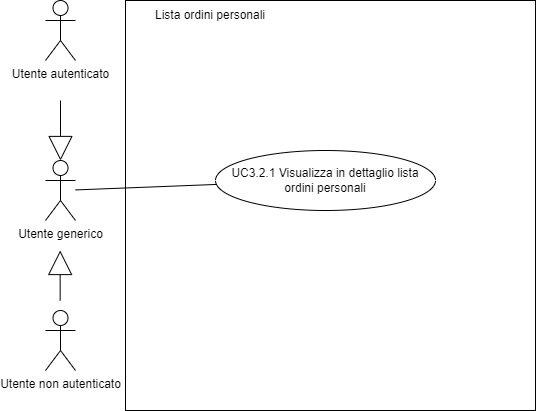
\includegraphics[scale=0.5]{usecase/tesi-uc322.drawio.png}
    \caption{Use Case - UC 3.2.1}
\end{figure}
\begin{itemize}
    \item \textbf{Descrizione:} L'utente visualizza la lista degli ordini personali in modalità dettaglio.
    \item \textbf{Attore Primario:}L'utente generico.
    \item \textbf{Precondizione:} L'utente si trova dentro la sezione lista ordini personali.
    \item \textbf{Postcondizione:} Viene visualizzato la lista degli ordini personali con i piatti in modalità dettaglio.
    \item \textbf{Scenrio principale:}
    \begin{itemize}
        \item L'utente si trova dentro la sezione gestione ordini personali;
        \item L'utente clicca sul bottone "lente" con il +;
        \item Viene mostrato la lista dei piatti ordinati personali in modalità dettaglio.
    \end{itemize}
\end{itemize}
\textbf{UC3.3.1 - Ricezione piatto}
\begin{figure}[H]
    \centering
    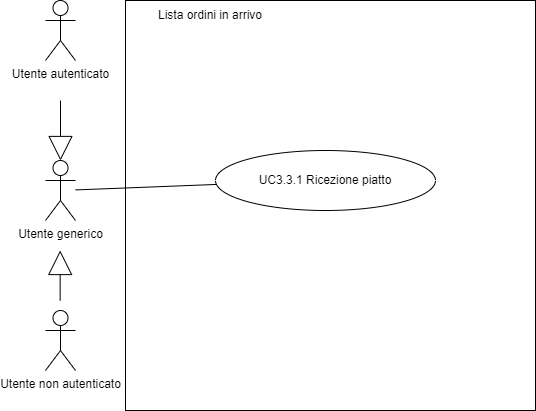
\includegraphics[scale=0.5]{usecase/tesi-uc333.drawio.png}
    \caption{Use Case - UC 3.3.1}
\end{figure}
\begin{itemize}
    \item \textbf{Descrizione:} L'utente marca un piatto in arrivo come ricevuto.
    \item \textbf{Attore Primario:}L'utente generico.
    \item \textbf{Precondizione:} L'utente si trova dentro la sezione gestione ordini in arrivo e ha almeno un piatto nella lista in arrivo.
    \item \textbf{Postcondizione:} L'utente marca il piatto come arrivato diminuendo di 1 la sua quantità.
    \item \textbf{Scenrio principale:}
    \begin{itemize}
        \item L'utente si trova dentro la sezione gestione lista ordini in arrivo;
        \item L'utente clicca sul bottone "v" di un piatto;
        \item Viene diminuito di 1 la sua quantità.
    \end{itemize}
    \item \textbf{Scenrio alternativo:}
    \begin{itemize}
        \item L'utente si trova dentro la sezione gestione lista ordini in arrivo;
        \item L'utente clicca sul bottone "v" di un piatto con quantità uguale a 1;
        \item Viene diminuito di 1 la quantità del piatto e viene disabilitato il bottone.
    \end{itemize}
\end{itemize}

\textbf{Utente non autenticato}\\
\textbf{UC4 - Area personale}
\begin{figure}[H]
    \centering
    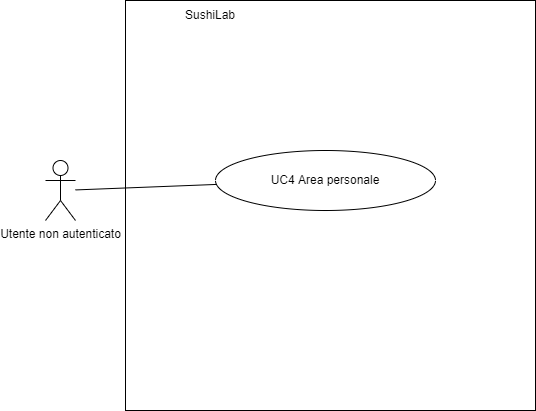
\includegraphics[scale=0.5]{usecase/tesi-uc4.drawio.png}
    \caption{Use Case - UC 4}
\end{figure}
\begin{itemize}
    \item \textbf{Descrizione:} L'utente visualizza la maschera dell'area personale.
    \item \textbf{Attore Primario:}L'utente non autenticato.
    \item \textbf{Precondizione:} L'utente si trova dentro la web-app sushiLab.
    \item \textbf{Postcondizione:} Viene visualizzato la maschera dell'area personale.
    \item \textbf{Scenrio principale:}
    \begin{itemize}
        \item L'utente si trova dentro il sistema;
        \item Viene mostrato la mascheradell'area personale.
    \end{itemize}
\end{itemize}
\textbf{UC4.1 - Registrazione}
\begin{figure}[H]
    \centering
    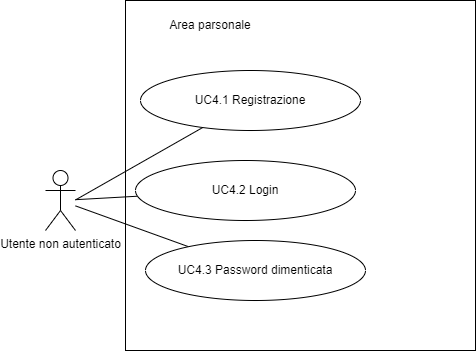
\includegraphics[scale=0.5]{usecase/tesi-uc41.drawio.png}
    \caption{Use Case - UC 4.1, UC 4.2, UC 4.3}
\end{figure}
\begin{itemize}
    \item \textbf{Descrizione:} L'utente viene registrato nella piattaforma.
    \item \textbf{Attore Primario:}L'utente non autenticato.
    \item \textbf{Precondizione:} L'utente si trova dentro la web-app sushiLab.
    \item \textbf{Postcondizione:} Viene salvato i dati dell'utente inseriti durante la fase di registrazione nel data-base.
    \item \textbf{Scenrio principale:}
    \begin{itemize}
        \item L'utente si trova dentro l'area personale;
        \item L'utente clicca sul bottone registrati;
        \item Vine mostrato il form di registrazione;
        \item L'utente inserisce l'email;
        \item L'utente inserisce la password;
        \item L'utente ripete la password;
        \item L'utente clicca sul bottone registrati;
        \item Viene registrato correttamente l'account.
    \end{itemize}
    % \item \textbf{Estensioni:}
    % \begin{itemize}
    %     \item L'utente inserisce l'email già esistente nel data-base;
    %     \item Non viene registrato l'acocunt.
    % \end{itemize}
\end{itemize}
\textbf{UC4.2 - Login}
\begin{itemize}
    \item \textbf{Descrizione:} L'utente effettua login nella piattaforma.
    \item \textbf{Attore Primario:} L'utente non autenticato.
    \item \textbf{Precondizione:} L'utente si trova dentro la web-app sushiLab.
    \item \textbf{Postcondizione:} Viene effettuato il login.
    \item \textbf{Scenrio principale:}
    \begin{itemize}
        \item L'utente si trova dentro l'area personale;
        \item L'utente inserisce l'email;
        \item L'utente inserisce la password;
        \item L'utente clicca sul bottone login;
        \item Viene effettuato il login correttamente.
    \end{itemize}
    % \item \textbf{Estensioni:}
    % \begin{itemize}
    %     \item L'utente inserisce l'email non esistente nel data-base o una password errata;
    %     \item Non viene effettuato il login.
    % \end{itemize}
\end{itemize}
\textbf{UC4.3 - Password dimenticata}
\begin{itemize}
    \item \textbf{Descrizione:} L'utente reimposta la password del proprio account.
    \item \textbf{Attore Primario:}L'utente non autenticato.
    \item \textbf{Precondizione:} L'utente si trova dentro la web-app sushiLab.
    \item \textbf{Postcondizione:} Viene aggiornato la nuova password nel data-base.
    \item \textbf{Scenrio principale:}
    \begin{itemize}
        \item L'utente si trova dentro l'area personale;
        \item L'utente clicca sul bottone password dimenticata;
        \item Vine mostrato il form di recupero password;
        \item L'utente inserisce l'email;
        \item L'utente clicca sul bottone ottieni codice;
        \item L'utente arriva nel secondo form tramite il link mandato tramite email;
        \item L'utente inserisce la password;
        \item L'utente ripete la password;
        \item L'utente clicca sul bottone cambia password;
        \item Viene cambiato correttamente la password.
    \end{itemize}
    % \item \textbf{Estensioni:}
    % \begin{itemize}
    %     \item L'utente inserisce l'email non esistente nel data-base;
    %     \item Non viene effettuato il cambio password.
    % \end{itemize}
\end{itemize}
% \textbf{UCE1 - Email}
% \begin{itemize}
%     \item \textbf{Descrizione:} L'utente reimposta la password del proprio account.
%     \item \textbf{Attore Primario:}L'utente non autenticato.
%     \item \textbf{Precondizione:} L'utente si trova dentro la web-app sushiLab.
%     \item \textbf{Postcondizione:} Viene aggiornato la nuova password nel data-base.
%     \item \textbf{Scenrio principale:}
%     \begin{itemize}
%         \item L'utente si trova dentro l'area personale;
%         \item L'utente clicca sul bottone password dimenticata;
%         \item Vine mostrato il form di recupero password;
%         \item L'utente inserisce l'email;
%         \item L'utente clicca sul bottone ottieni codice;
%         \item L'utente arriva nel secondo form tramite il link mandato tramite email;
%         \item L'utente inserisce la password;
%         \item L'utente ripete la password;
%         \item L'utente clicca sul bottone cambia password;
%         \item Viene cambiato correttamente la password.
%     \end{itemize}
% \end{itemize}
\textbf{Utente autenticato}\\
\textbf{UC4.4 - Logout}
\begin{figure}[H]
    \centering
    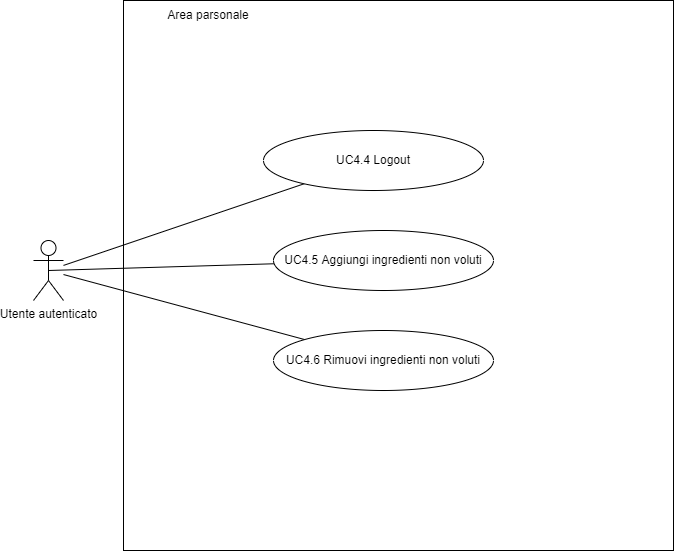
\includegraphics[scale=0.5]{usecase/tesi-uc42.drawio.png}
    \caption{Use Case - UC 4.4, UC4.5, UC4.6}
\end{figure}
\begin{itemize}
    \item \textbf{Descrizione:} L'utente effettua logout.
    \item \textbf{Attore Primario:}L'utente autenticato.
    \item \textbf{Precondizione:} L'utente si trova dentro la web-app sushiLab ed ha effettuato il login.
    \item \textbf{Postcondizione:} Viene effettuato il logout.
    \item \textbf{Scenrio principale:}
    \begin{itemize}
        \item L'utente si trova dentro l'area personale;
        \item L'utente clicca sul bottone logout;
        \item Viene effettuato il logout dell'utente.
    \end{itemize}
\end{itemize}
\textbf{UC4.5 - Aggiungi ingredienti non voluti}
\begin{itemize}
    \item \textbf{Descrizione:} L'utente inserisce un ingrediente nella blacklist.
    \item \textbf{Attore Primario:}L'utente autenticato.
    \item \textbf{Precondizione:} L'utente si trova dentro la web-app sushiLab  ha effettuato il login.
    \item \textbf{Postcondizione:} Viene inserito l'ingrediente nella blacklist.
    \item \textbf{Scenrio principale:}
    \begin{itemize}
        \item L'utente si trova dentro l'area personale;
        \item L'utente clicca sul bottone blacklist ingredienti;
        \item L'utente inserisce il nome del ingrediente;
        \item L'utente clicca sul bottone +;
        \item Viene inserito ingrediente nella blacklist.
    \end{itemize}
\end{itemize}
\textbf{UC4.6 - Rimuovi ingredienti non voluti}
\begin{itemize}
    \item \textbf{Descrizione:} L'utente rimuove un ingrediente dalla blacklist.
    \item \textbf{Attore Primario:}L'utente autenticato.
    \item \textbf{Precondizione:} L'utente si trova dentro la web-app sushiLab  ha effettuato il login.
    \item \textbf{Postcondizione:} Viene rimosso l'ingrediente dalla blacklist.
    \item \textbf{Scenrio principale:}
    \begin{itemize}
        \item L'utente si trova dentro l'area personale;
        \item L'utente clicca sul bottone blacklist ingredienti;
        \item L'utente clicca sul bottone - di un ingrediente già esistente;
        \item Viene rimosso ingrediente dalla blacklist.
    \end{itemize}
\end{itemize}
\textbf{UC1.7 - Aggiungi preferiti}
\begin{figure}[H]
    \centering
    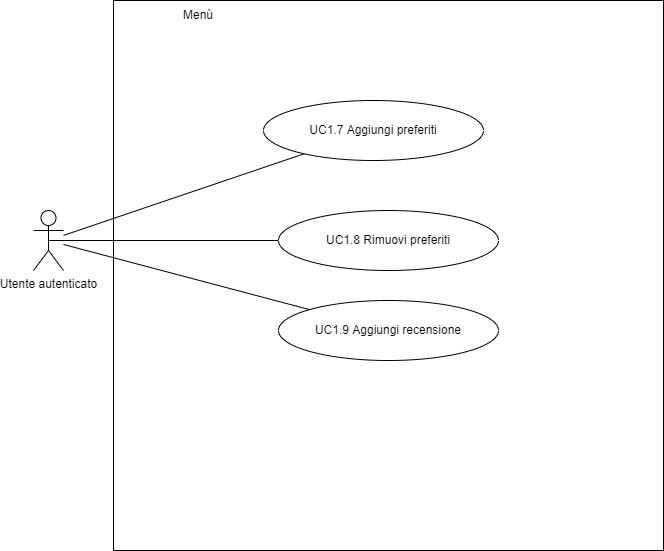
\includegraphics[scale=0.5]{usecase/tesi-uc111.drawio.png}
    \caption{Use Case - UC 1.7, UC1.8, UC1.9}
\end{figure}
\begin{itemize}
    \item \textbf{Descrizione:} L'utente aggiunge un piatto nella lista dei preferiti.
    \item \textbf{Attore Primario:}L'utente autenticato.
    \item \textbf{Precondizione:} L'utente si trova dentro nella sezione menù, lista ordini personali o lista ordini in arrivo.
    \item \textbf{Postcondizione:} Viene inserito il piatto nei preferiti.
    \item \textbf{Scenrio principale:}
    \begin{itemize}
        \item L'utente si trova nella sezione menù, lista ordini personali o lista ordini in arrivo;
        \item L'utente clicca sul bottone "cuoricino grigio";
        \item Viene inserito il piatto nella lista dei preferiti.
    \end{itemize}
\end{itemize}
\textbf{UC1.8 - Rimuovi preferiti}
\begin{itemize}
    \item \textbf{Descrizione:} L'utente rimuove un piatto nella lista dei preferiti.
    \item \textbf{Attore Primario:}L'utente autenticato.
    \item \textbf{Precondizione:} L'utente si trova dentro nella sezione menù, lista ordini personali, lista ordini in arrivo o lista preferiti.
    \item \textbf{Postcondizione:} Viene rimosso il piatto dalla lista dei preferiti.
    \item \textbf{Scenrio principale:}
    \begin{itemize}
        \item L'utente si trova nella sezione menù;
        \item L'utente clicca sul bottone "cuoricino rosa";
        \item Viene rimosso il piatto nella lista dei preferiti.
    \end{itemize}
\end{itemize}
\textbf{UC1.9 - Aggiungi recensione}
\begin{itemize}
    \item \textbf{Descrizione:} L'utente Aggiungi una recensione per un piatto.
    \item \textbf{Attore Primario:}L'utente autenticato.
    \item \textbf{Precondizione:} L'utente ha selezionato un piatto e il piatto è in modalità dettaglio.
    \item \textbf{Postcondizione:} Viene aggiornato la recensione del piatto.
    \item \textbf{Scenrio principale:}
    \begin{itemize}
        \item L'utente ha selezionato un piatto e il piatto è in modificata dettaglio;
        \item L'utente clicca su una delle 5 stelle;
        \item Viene inserito la recensione del piatto.
    \end{itemize}
\end{itemize}
\textbf{UC5 - Visualizza lista preferiti}
\begin{figure}[H]
    \centering
    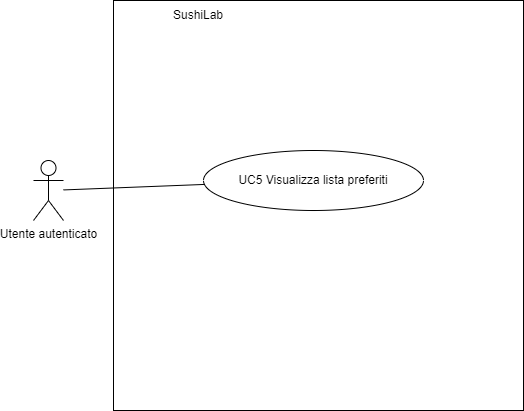
\includegraphics[scale=0.5]{usecase/tesi-uc5.drawio.png}
    \caption{Use Case - UC 5}
\end{figure}
\begin{itemize}
    \item \textbf{Descrizione:} L'utente visualizza la lista dei preferiti.
    \item \textbf{Attore Primario:}L'utente autenticato.
    \item \textbf{Precondizione:} L'utente si trova dentro la web-app sushiLab ed ha effettuato il login.
    \item \textbf{Postcondizione:} Viene mostrato la lista dei preferiti.
    \item \textbf{Scenrio principale:}
    \begin{itemize}
        \item L'utente si trova dentro la web-app;
        \item L'utente entra nalla sezione lista preferiti;
        \item Viene mostrato la lista dei preferiti.
    \end{itemize}
\end{itemize}
